\section{Contemplation of a fixed black hole}

\subsection{Approximation from Schwarzschild to Rindler}
Upto now we still considered the quantum field theory and classical black holes apart from each other. Combining them would require a theory of quantum gravity on which i will not go deeper in this thesis. But we can start with a much simpler problem that would be the quantum field theory in a fixed black hole backround. Physically this means, that we're sending $G$ to zero and the mass of the black hole $M$ to infinity so that the Schwarzschild radius $r_s = 2GM$ ist fixed. This can be assured by sending $\frac{M}{m_p}$ to infinity, where $m_p =\frac{1}{\sqrt{8\pi G}}$ is the Planck mass. 

This approximation is justified, which we can see by the example of a black hole with the mass of our sun:
	\begin{align}
		\frac{m_p}{M_{solar}} \approx 10^{-38}
	\end{align}	 
In this type of scale, the Schwarzschild radius is in order of kilometers (sun: $r_s=3 \unit{km}$) where we could imagine doing experiments. 

Now we must descide, which geometry we use. Either the two-sided Schwarzschild geometry or the one-sided collapse geometry. The disadvantage of the latter is, that it is only Schwarzschild after the infalling matter has gone in. So for avoiding the infalling shell problem, we use the former. 
The Schwarzschild geometry is approximatly the region of Minkowski space which is near the Rindler horizon in the Rindler decomposition, if $r \approx 1$ and the angular arrangement is not quite too big. We now sketch this for the right exterior ($r>1$) by using the tortoise coordinate from \eqref{r_*tortoise}:
	\begin{align*}
		r_*=r + log(r-1)
	\end{align*}
The Schwarzschild metric then is
	\begin{align}
		\diff s^2=\frac{r-1}{r}\left(-\diff t^2 + \diff r^2_*\right) + r^2 \diff \Omega^2_2
	\end{align}
Now let's say $y_1=\theta, y_2=\varphi$ where the two angulars are orthogonal coordinates on the sphere. Near the horizon $r\approx1$ the metric then looks like 
	\begin{align}
		\diff s^2 \approx e^{r_* - 1} \left(-\diff t^2 + \diff r^2_*\right) + \diff \vec{y}^2
	\end{align}
This quite resembles the right Rindler wedge metric. It even becomes equal, if we insert
	\begin{align}
		\begin{split}
			r_*&= 2\xi_R + 1 - \log 4 \\
			t &= 2\tau_R
		\end{split}
	\end{align}
which leads to
	\begin{align*}
		&\Rightarrow &
		\diff t^2 &= 4 \diff \tau_R^2 & \diff r_*^2 &= 4 \diff \xi_R^2 &e^{r_* -1} &= e^{2\xi_R + 1 - 1 - \log 4} & \diff \vec{y}^2 &= \diff \vec{y}^2
	\end{align*}
and finaly like in \eqref{Rindler_metric}
	\begin{align*}
		\diff s^2 = e^{2\xi_R} (-\diff \tau_R^2 + \diff \xi_R^2) + \diff \vec{y}^2 
	\end{align*}
How this looks like in Penrose diagrams if we do the same thing for the other three wedges too, can be seen in \textbf{Figure \ref{approximation}}.
\begin{figure}[tb]
	\begin{center}
		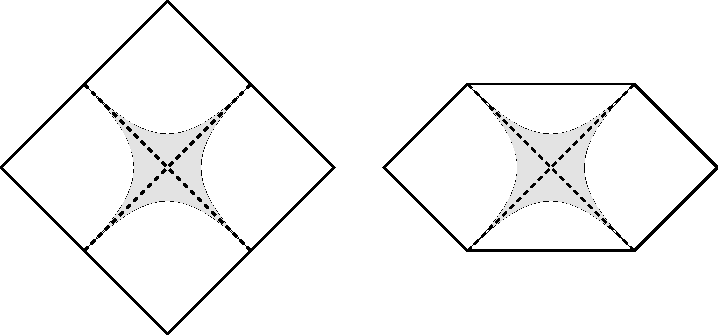
\includegraphics[scale=1]{rindsch} \label{approximation}
		\caption{At the left, one can see the Rindler Penrose, at the right there is the Schwarzschild Penrose. The two grey regions in the middle are the regions near the horizon. As you can see, they approximate each other well. Note that a $\mathds{R}^2$ is suppressed at each point instead of $\mathds{S}^2$ which is why the left Penrose doesn't look like the Minkowski Penrose in \textbf{Figure \ref{flatpenrose}}.}\label{approximation}
	\end{center}
\end{figure}
The outcome of this is, that for every initial state in a Schwarzschild geometry the left and right exteriors must be thermally entangled, assumed that the Schwarzschild looks like Minkowski space near them. 